\begin{figure}[!h]
  %\centering
  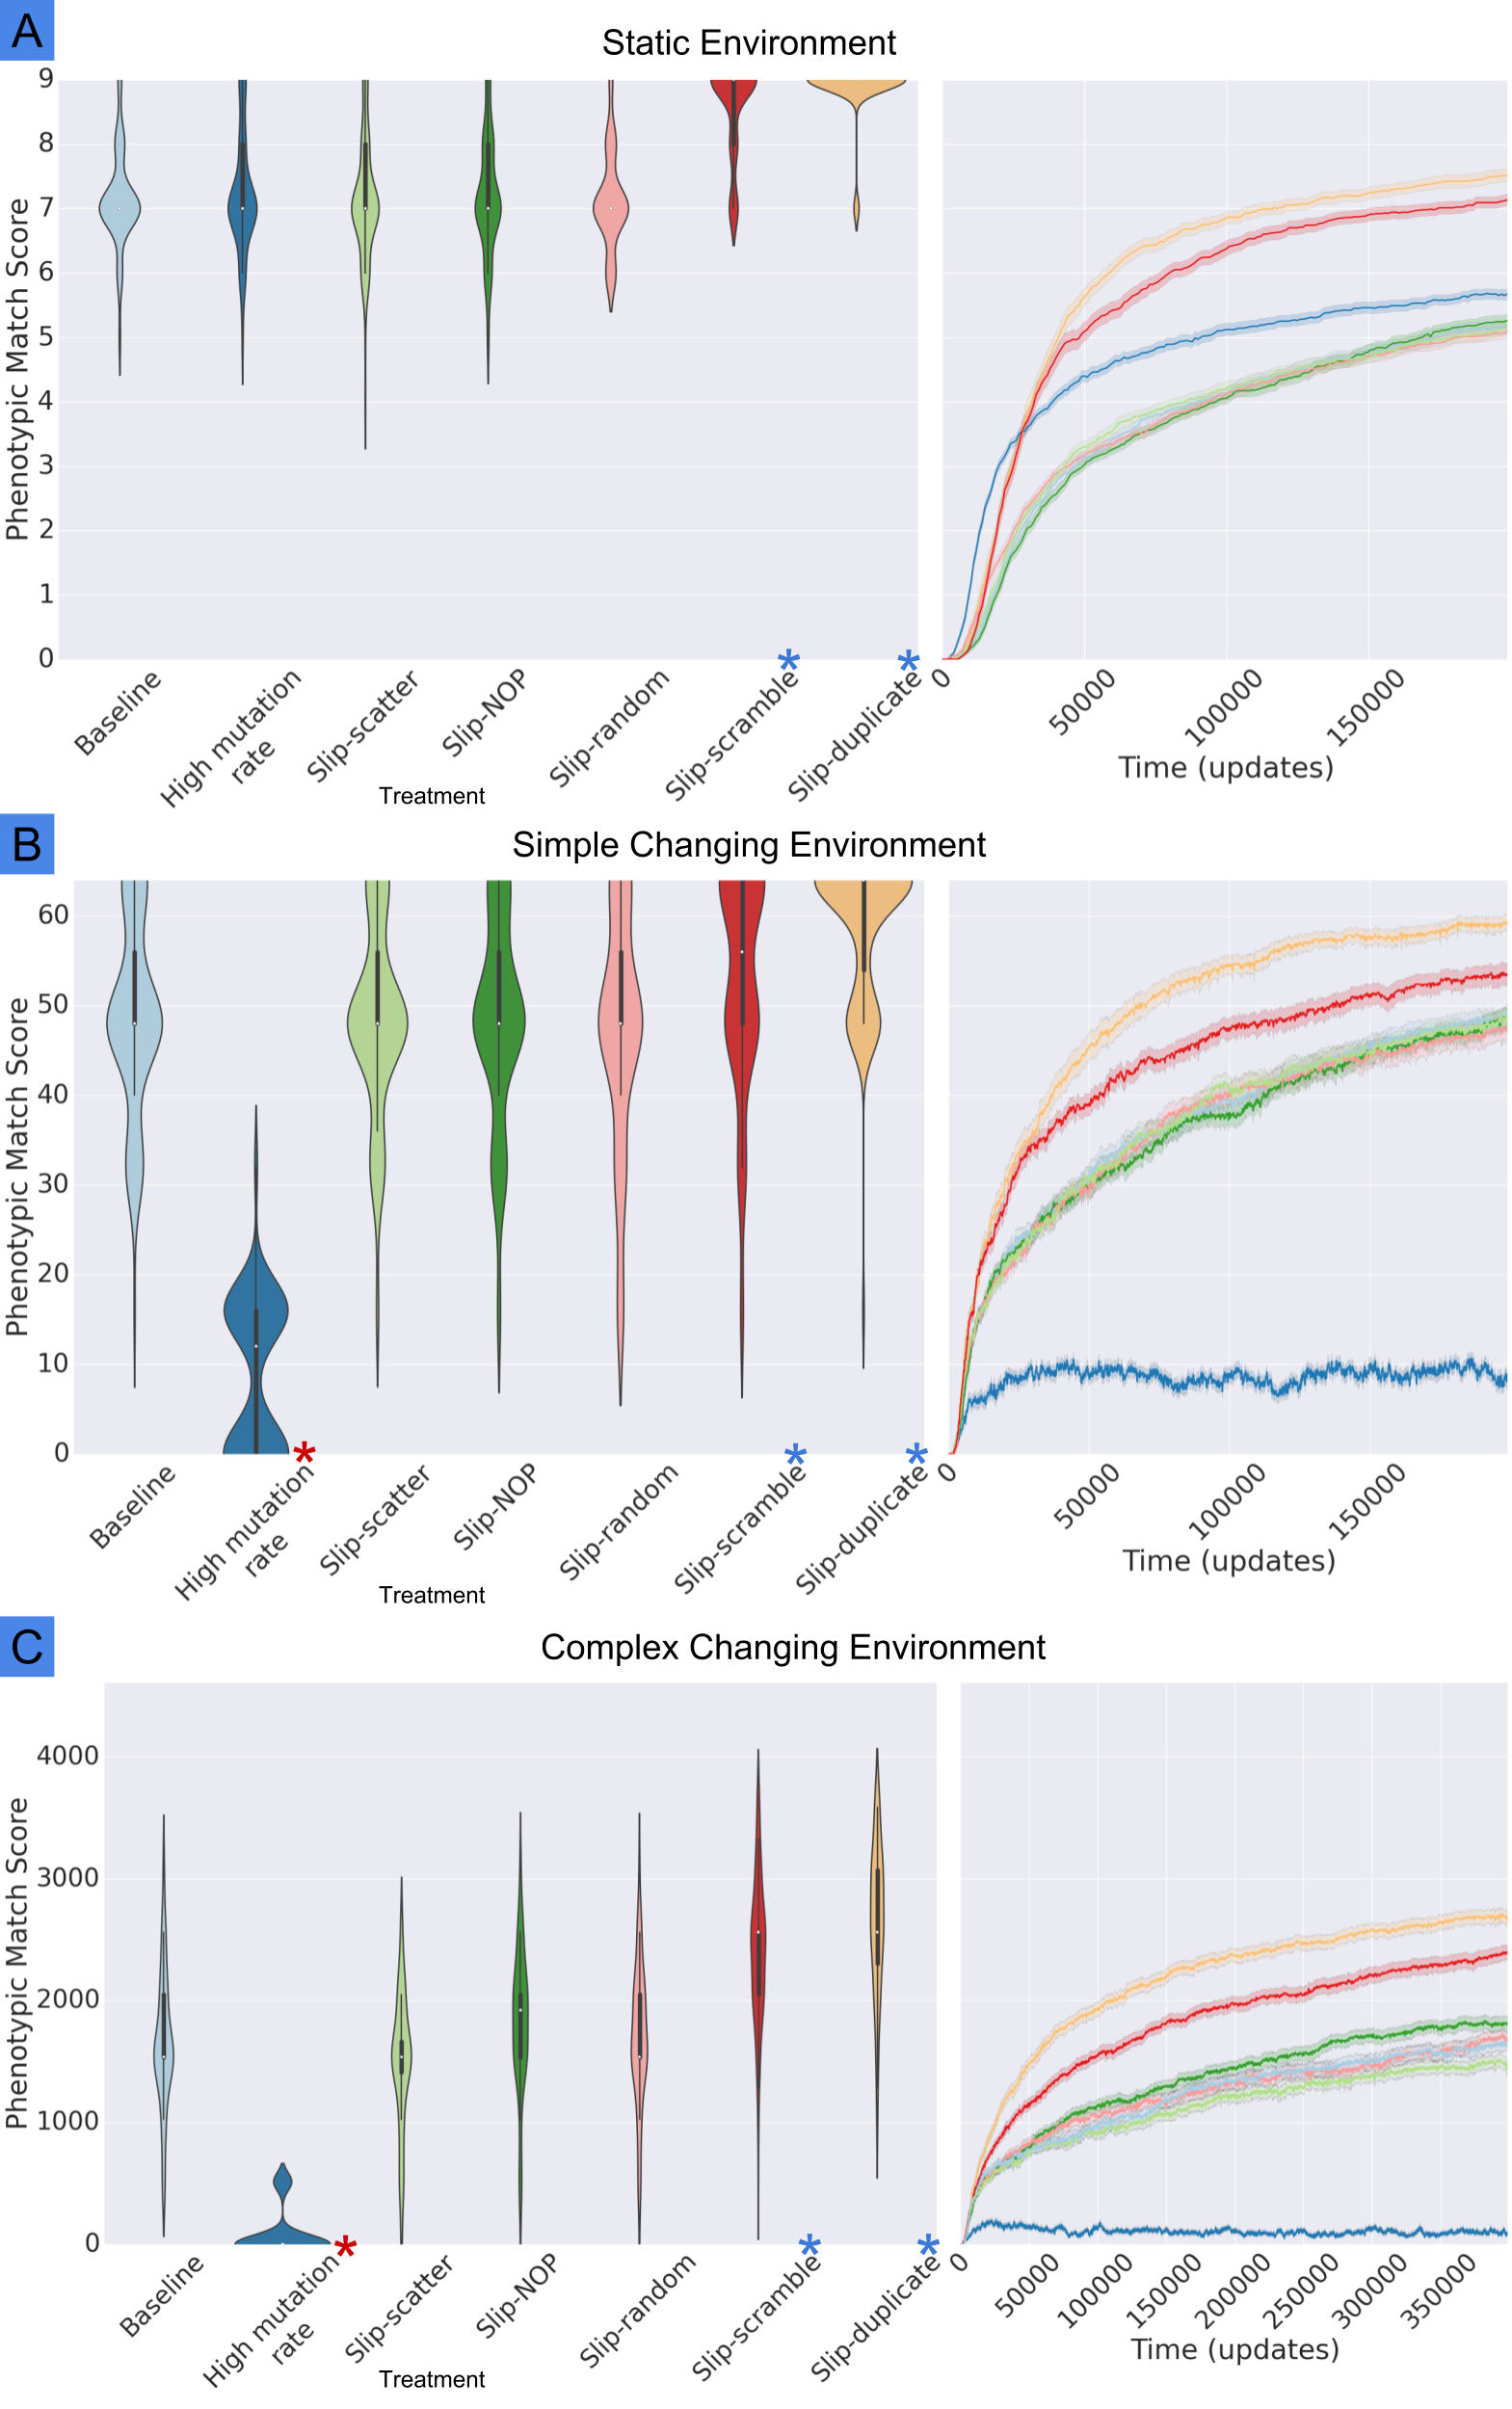
\includegraphics[width=\columnwidth]{imgs/results_panels.png}
  \caption{\small Experimental results from all three environments: A) static environment, B) simple changing environment, and C) complex changing environment. The violin plots for each environment indicate the phenotypic adaptation scores for final dominants in the static environment and for the ancestors of final dominants that existed 1000 updates prior to the end of a trial in the simple and complex changing environments. Each time series shows the phenotypic adaptation scores for the lineages of final dominant organisms over time. The colors in each time series correspond to the colors in the violin plots. Treatments that have significantly higher phenotypic adaptation scores than the baseline treatment are marked with blue *, and treatments that have significantly lower phenotypic adaptation scores than the baseline treatment are marked with red *.  }
  \label{fig:results_panels}
\end{figure}
